\newcommand{\adwareTagResultsAucTable}{
    \begin{table}[H]
        \centering
        \begin{tabular}{|p{2,8cm}||p{2,8cm} p{2,8cm} p{2,8cm}|}
            \hline
            Adware Tag & ALOHA & Joint Embedding & Proposed Model \\
            \hline
            AUC-ROC & 0.973$\pm$0.000 & 0.969$\pm$0.001 & \textBF{0.974$\pm$0.002} \\
            \hline
        \end{tabular}
        \caption{AUC-ROC (Area Under Curve) of the different models for the \textbf{Adware Tag} prediction task. Results were aggregated over \textBF{3} training runs with different weight initializations and minibatch orderings. Best results are shown in \textbf{bold}.} \label{tab:adwareTag_auc}
    \end{table}
}

\newcommand{\adwareTagResultsAtFprTable}{
    \begin{center}
        \begin{longtable}[c]{|p{3,2cm}||p{1,8cm} p{1,8cm} p{1,8cm} p{1,8cm} p{1,8cm}|}
            \hline
            Adware Tag & \multicolumn{5}{c|}{{FPR}} \\
            & $10^{-5}$ & $10^{-4}$ & $10^{-3}$ & $10^{-2}$ & $10^{-1}$ \\
            \hline
            \endfirsthead

            \caption*{\raggedright ...continued from previous page} \\
            \hline
            Adware Tag & \multicolumn{5}{c|}{\textbf{FPR}} \\
            & $10^{-5}$ & $10^{-4}$ & $10^{-3}$ & $10^{-2}$ & $10^{-1}$ \\
            \hline
            \endhead

            \caption*{\raggedleft ...continued on next page} \\
            \endfoot

            \caption{Mean and standard deviation results (TPR, Accuracy, Recall, Precision and F1-Score) of the different models for the \textbf{Adware Tag} prediction task at different \textbf{FPR}s (\textit{False Positive Rates}). Results were aggregated over \textBF{3} training runs with different weight initializations and minibatch orderings. Best results are shown in \textbf{bold}. Under \textbf{TPR} results are also presented the percentage reduction in mean detection error and in ROC curve standard deviation introduced by the \textit{Proposed Model} with respect to both \textit{ALOHA} model and \textit{Joint Embedding}.} \label{tab:adwareTag_results_at_fpr} \\
            \endlastfoot

            \multicolumn{6}{|c|}{\textbf{TPR}} \\
            \hline
            ALOHA & 0.129$\pm$0.017 & \textBF{0.256$\pm$0.029} & 0.453$\pm$0.047 & \textBF{0.719$\pm$0.006} & 0.934$\pm$0.010 \\
            Joint Embedding & 0.101$\pm$0.042 & 0.194$\pm$0.056 & \textBF{0.481$\pm$0.047} & 0.688$\pm$0.012 & 0.924$\pm$0.001 \\
            Proposed Model & \textBF{0.146$\pm$0.031} & 0.254$\pm$0.058 & 0.426$\pm$0.026 & 0.662$\pm$0.027 & \textBF{0.941$\pm$0.001} \\
            \hline
            Error Reduction wrt \newline ALOHA & 2.0\% & -0.3\% & -4.9\% & -20.3\% & 10.6\% \\
            Error Reduction wrt \newline Joint Embedding & 5.0\% & 7.4\% & -10.6\% & -8.3\% & 22.4\% \\
            \hline
            Std Reduction wrt \newline ALOHA & -82.4\% & -100.0\% & 44.7\% & -350.0\% & 90.0\% \\
            Std Reduction wrt \newline Joint Embedding & 26.2\% & -3.6\% & 44.7\% & -125.0\% & 0.0\% \\
            \hline
            \multicolumn{6}{|c|}{\textbf{Accuracy}} \\
            \hline
            ALOHA & 0.950$\pm$0.001 & \textBF{0.957$\pm$0.002} & 0.968$\pm$0.003 & \textBF{0.974$\pm$0.000} & 0.902$\pm$0.001 \\
            Joint Embedding & 0.948$\pm$0.002 & 0.954$\pm$0.003 & \textBF{0.969$\pm$0.003} & 0.973$\pm$0.001 & 0.901$\pm$0.000 \\
            Proposed Model & \textBF{0.951$\pm$0.002} & 0.957$\pm$0.003 & 0.966$\pm$0.001 & 0.971$\pm$0.002 & \textBF{0.902$\pm$0.000} \\
            \hline
            \multicolumn{6}{|c|}{\textbf{Recall}} \\
            \hline
            ALOHA & 0.129$\pm$0.017 & \textBF{0.256$\pm$0.029} & 0.453$\pm$0.047 & \textBF{0.719$\pm$0.006} & 0.934$\pm$0.010 \\
            Joint Embedding & 0.101$\pm$0.042 & 0.194$\pm$0.056 & \textBF{0.481$\pm$0.047} & 0.688$\pm$0.012 & 0.924$\pm$0.001 \\
            Proposed Model & \textBF{0.146$\pm$0.031} & 0.254$\pm$0.058 & 0.426$\pm$0.026 & 0.662$\pm$0.027 & \textBF{0.941$\pm$0.001} \\
            \hline
            \multicolumn{6}{|c|}{\textbf{Precision}} \\
            \hline
            ALOHA & \textBF{0.999$\pm$0.000} & \textBF{0.994$\pm$0.001} & 0.965$\pm$0.004 & \textBF{0.814$\pm$0.001} & 0.363$\pm$0.003 \\
            Joint Embedding & 0.998$\pm$0.001 & 0.991$\pm$0.002 & \textBF{0.967$\pm$0.003} & 0.808$\pm$0.003 & 0.361$\pm$0.000 \\
            Proposed Model & \textBF{0.999$\pm$0.000} & 0.993$\pm$0.002 & 0.963$\pm$0.002 & 0.801$\pm$0.007 & \textBF{0.365$\pm$0.000} \\
            \hline
            \multicolumn{6}{|c|}{\textbf{F1 Score}} \\
            \hline
            ALOHA & 0.228$\pm$0.027 & \textBF{0.406$\pm$0.037} & 0.615$\pm$0.045 & \textBF{0.764$\pm$0.004} & 0.523$\pm$0.004 \\
            Joint Embedding & 0.181$\pm$0.071 & 0.321$\pm$0.077 & \textBF{0.641$\pm$0.043} & 0.743$\pm$0.008 & 0.519$\pm$0.000 \\
            Proposed Model & \textBF{0.254$\pm$0.046} & 0.401$\pm$0.075 & 0.590$\pm$0.025 & 0.725$\pm$0.019 & \textBF{0.526$\pm$0.001} \\
            \hline
        \end{longtable}
    \end{center}
}

\newcommand{\adwareTagResultsSummaryTable}{
    \begin{table}[H]
        \centering
        \begin{tabular}{|p{3,2cm}||p{1,8cm} p{1,8cm} p{1,8cm} p{1,8cm} p{1,8cm}|}
            \hline
            \multicolumn{6}{|c|}{Adware Tag (at FPR $=1\%$)} \\
            \hline
            Model & TPR & Accuracy & Precision & Recall & F1 score \\
            \hline
            ALOHA & \textBF{0.719$\pm$0.006} & \textBF{0.974$\pm$0.000} & \textBF{0.814$\pm$0.001} & \textBF{0.719$\pm$0.006} & \textBF{0.764$\pm$0.004} \\
            Joint Embedding & 0.688$\pm$0.012 & 0.973$\pm$0.001 & 0.808$\pm$0.003 & 0.688$\pm$0.012 & 0.743$\pm$0.008 \\
            Proposed Model & 0.662$\pm$0.027 & 0.971$\pm$0.002 & 0.801$\pm$0.007 & 0.662$\pm$0.027 & 0.725$\pm$0.019 \\
            \hline
        \end{tabular}
        \caption{Summary of the mean and standard deviation results of the different models for the \textbf{Adware Tag} prediction task at \textbf{FPR} $=1\%$. Results were aggregated over \textBF{3} training runs with different weight initializations and minibatch orderings. Best results are shown in \textbf{bold}.} \label{tab:adwareTag_result_summary}
    \end{table}
}

\newcommand{\adwareTagRocAloha}{
    \begin{figure}[H]
        \vspace*{-0.5cm}
        \centering
        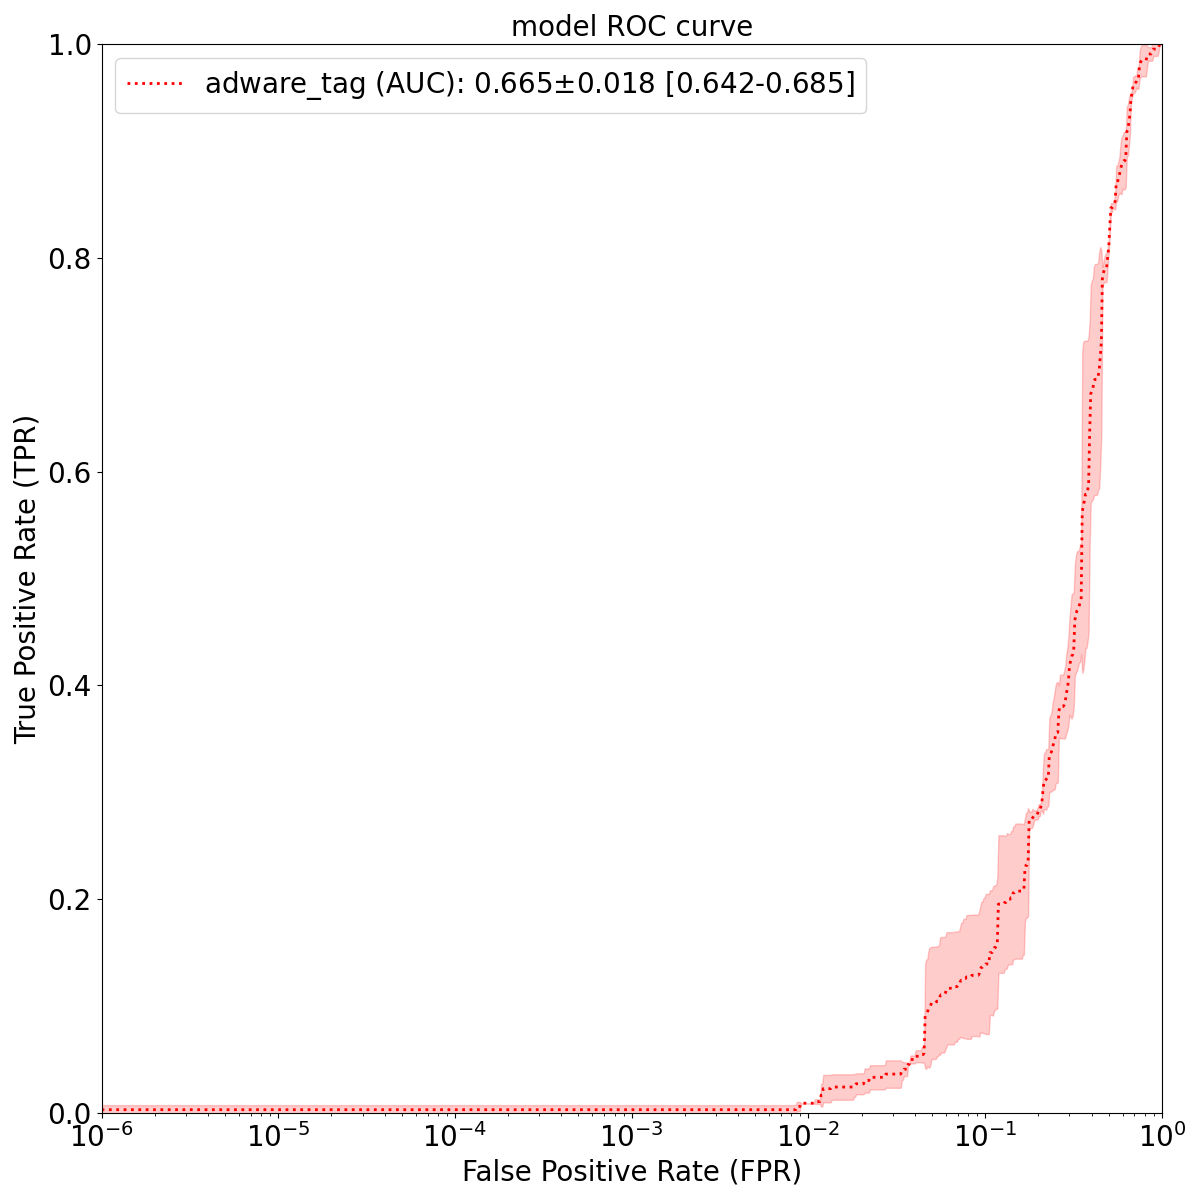
\includegraphics[width=0.6\textwidth]{./results/adware_tag_roc_aloha.png}
        \vspace*{-0.2cm}
        \caption{ROC curve and AUC statistics of \textBF{ALOHA} model for the \textbf{Adware Tag}. The line represents the \textit{mean} TPR at a given FPR, while the shaded region represents the \textit{standard deviation}. Statistics were computed over \textBF{3} training runs, each with random parameter initialization.}
        \label{fig:adwareTagRocAloha}
    \end{figure}
}

\newcommand{\adwareTagRocJointEmbedding}{
    \begin{figure}[H]
        \vspace*{-0.5cm}
        \centering
        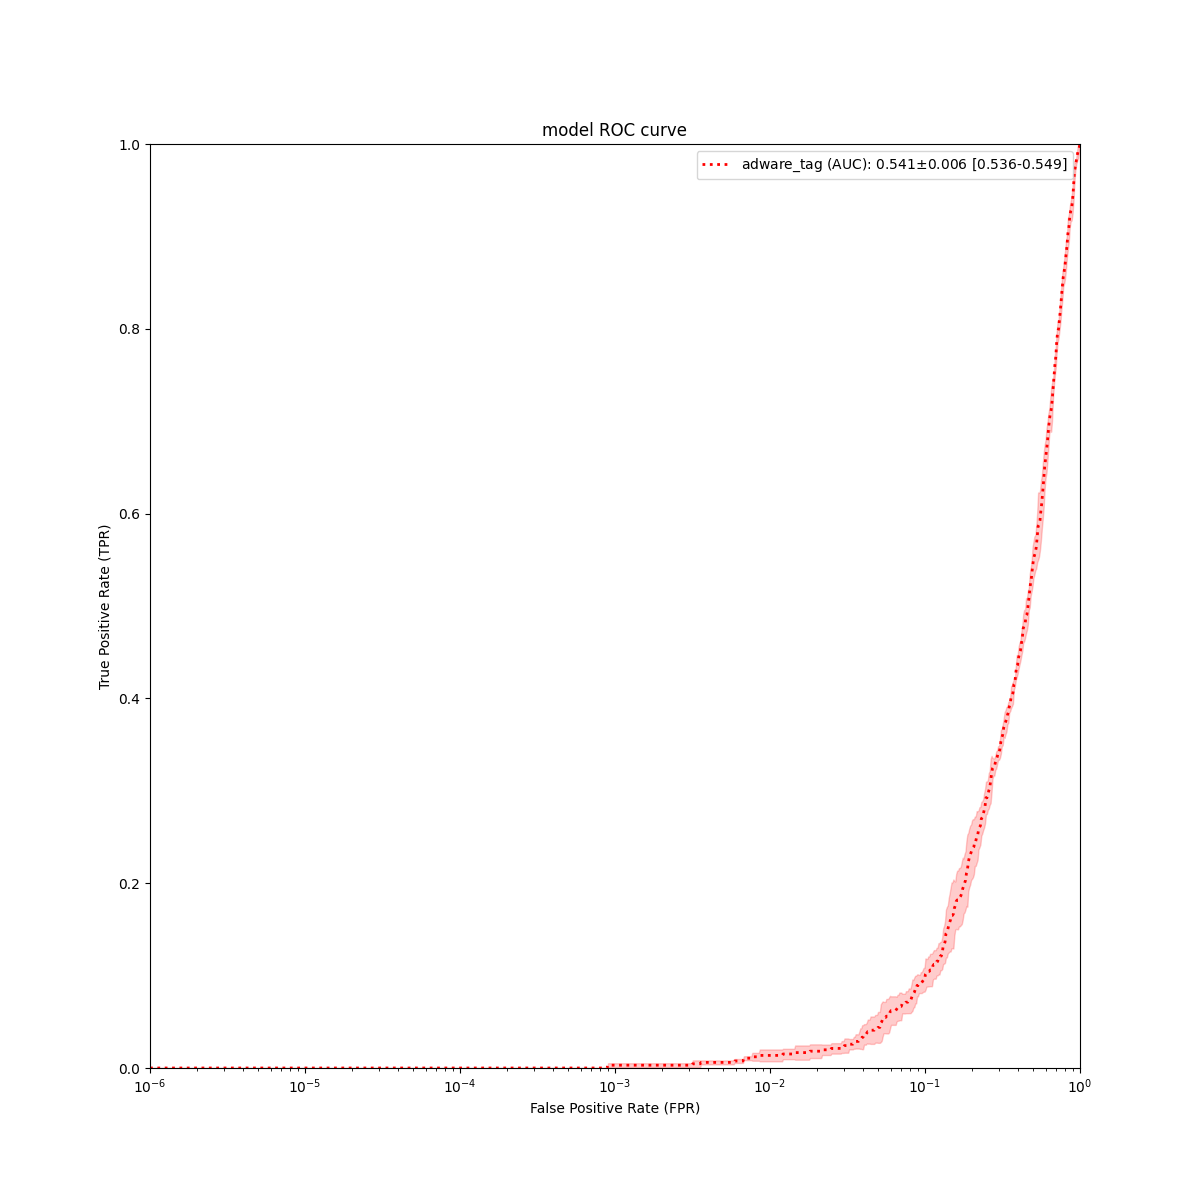
\includegraphics[width=0.6\textwidth]{./results/adware_tag_roc_jointEmbedding.png}
        \vspace*{-0.2cm}
        \caption{ROC curve and AUC statistics of \textBF{Joint Embedding} model for the \textbf{Adware Tag}. The line represents the \textit{mean} TPR at a given FPR, while the shaded region represents the \textit{standard deviation}. Statistics were computed over \textBF{3} training runs, each with random parameter initialization.}
        \label{fig:adwareTagRocJointEmbedding}
    \end{figure}
}

\newcommand{\adwareTagRocProposedMethod}{
    \begin{figure}[H]
        \vspace*{-0.5cm}
        \centering
        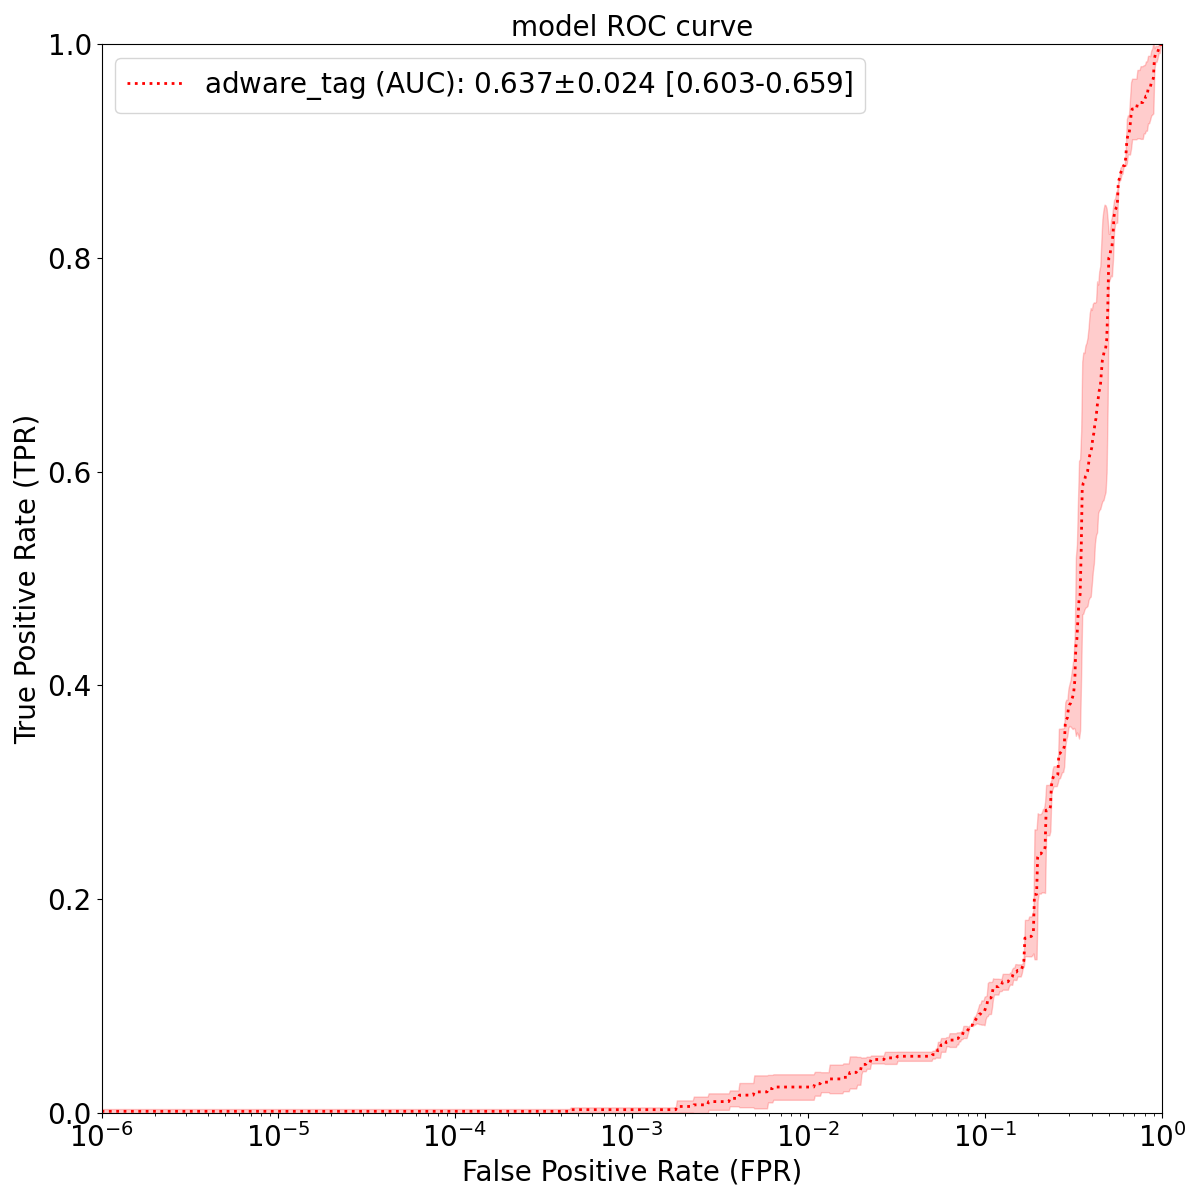
\includegraphics[width=0.6\textwidth]{./results/adware_tag_roc_proposedModel.png}
        \vspace*{-0.2cm}
        \caption{ROC curve and AUC statistics of \textBF{Proposed Model} for the \textbf{Adware Tag}. The line represents the \textit{mean} TPR at a given FPR, while the shaded region represents the \textit{standard deviation}. Statistics were computed over \textBF{3} training runs, each with random parameter initialization.}
        \label{fig:adwareTagRocProposedModel}
    \end{figure}
}
